%% uncomment to list all files in log
%\listfiles

\documentclass[12pt]{report}


\usepackage{fontspec}

%\setmainfont[Scale=MatchLowercase]{Lucida Bright}
%\setmonofont{FreeMono}
%\setmonofont{Source Code Pro}
\setmonofont[Scale=MatchLowercase]{Ubuntu Mono}

\usepackage[headings]{fullpage}

% national use characters 
%\usepackage{inputenc}

% ams mathematical symbols
\usepackage{amsmath,amssymb}

% added to support pandoc highlighting
\usepackage{microtype}

\usepackage{makeidx}

% add index and bibliographies to table of contents
\usepackage[nottoc]{tocbibind}

% postscript courier and times in place of cm fonts
%\usepackage{courier}
%\usepackage{times}

% extended coloring
\usepackage{color}
\usepackage[table,dvipsnames]{xcolor}
\usepackage{colortbl}

% advanced date formating
\usepackage{datetime}

%support pandoc code highlighting
\usepackage{fancyvrb}
\DefineShortVerb[commandchars=\\\{\}]{\|}
\DefineVerbatimEnvironment{Highlighting}{Verbatim}{commandchars=\\\{\}}
% Add ',fontsize=\small' for more characters per line

%tango style colors
% \usepackage{framed}
% \definecolor{shadecolor}{RGB}{255,255,255}
% \newenvironment{Shaded}{\begin{snugshade}}{\end{snugshade}}
% \newcommand{\KeywordTok}[1]{\textcolor[rgb]{0.13,0.29,0.53}{\textbf{{#1}}}}
% \newcommand{\DataTypeTok}[1]{\textcolor[rgb]{0.13,0.29,0.53}{{#1}}}
% \newcommand{\DecValTok}[1]{\textcolor[rgb]{0.00,0.00,0.81}{{#1}}}
% \newcommand{\BaseNTok}[1]{\textcolor[rgb]{0.00,0.00,0.81}{{#1}}}
% \newcommand{\FloatTok}[1]{\textcolor[rgb]{0.00,0.00,0.81}{{#1}}}
% \newcommand{\CharTok}[1]{\textcolor[rgb]{0.31,0.60,0.02}{{#1}}}
% \newcommand{\StringTok}[1]{\textcolor[rgb]{0.31,0.60,0.02}{{#1}}}
% \newcommand{\CommentTok}[1]{\textcolor[rgb]{0.56,0.35,0.01}{\textit{{#1}}}}
% \newcommand{\OtherTok}[1]{\textcolor[rgb]{0.56,0.35,0.01}{{#1}}}
% \newcommand{\AlertTok}[1]{\textcolor[rgb]{0.94,0.16,0.16}{{#1}}}
% \newcommand{\FunctionTok}[1]{\textcolor[rgb]{0.00,0.00,0.00}{{#1}}}
% \newcommand{\RegionMarkerTok}[1]{{#1}}
% \newcommand{\ErrorTok}[1]{\textbf{{#1}}}
% \newcommand{\NormalTok}[1]{{#1}}

%espresso style colors
% \usepackage{framed}
% \definecolor{shadecolor}{RGB}{42,33,28}
% \newenvironment{Shaded}{\begin{snugshade}}{\end{snugshade}}
% \newcommand{\KeywordTok}[1]{\textcolor[rgb]{0.26,0.66,0.93}{\textbf{{#1}}}}
% \newcommand{\DataTypeTok}[1]{\textcolor[rgb]{0.74,0.68,0.62}{\underline{{#1}}}}
% \newcommand{\DecValTok}[1]{\textcolor[rgb]{0.27,0.67,0.26}{{#1}}}
% \newcommand{\BaseNTok}[1]{\textcolor[rgb]{0.27,0.67,0.26}{{#1}}}
% \newcommand{\FloatTok}[1]{\textcolor[rgb]{0.27,0.67,0.26}{{#1}}}
% \newcommand{\CharTok}[1]{\textcolor[rgb]{0.02,0.61,0.04}{{#1}}}
% \newcommand{\StringTok}[1]{\textcolor[rgb]{0.02,0.61,0.04}{{#1}}}
% \newcommand{\CommentTok}[1]{\textcolor[rgb]{0.00,0.40,1.00}{\textit{{#1}}}}
% \newcommand{\OtherTok}[1]{\textcolor[rgb]{0.74,0.68,0.62}{{#1}}}
% \newcommand{\AlertTok}[1]{\textcolor[rgb]{1.00,1.00,0.00}{{#1}}}
% \newcommand{\FunctionTok}[1]{\textcolor[rgb]{1.00,0.58,0.35}{\textbf{{#1}}}}
% \newcommand{\RegionMarkerTok}[1]{\textcolor[rgb]{0.74,0.68,0.62}{{#1}}}
% \newcommand{\ErrorTok}[1]{\textcolor[rgb]{0.74,0.68,0.62}{\textbf{{#1}}}}
% \newcommand{\NormalTok}[1]{\textcolor[rgb]{0.74,0.68,0.62}{{#1}}}

%kete style colors
% \newenvironment{Shaded}{}{}
% \newcommand{\KeywordTok}[1]{\textbf{{#1}}}
% \newcommand{\DataTypeTok}[1]{\textcolor[rgb]{0.50,0.00,0.00}{{#1}}}
% \newcommand{\DecValTok}[1]{\textcolor[rgb]{0.00,0.00,1.00}{{#1}}}
% \newcommand{\BaseNTok}[1]{\textcolor[rgb]{0.00,0.00,1.00}{{#1}}}
% \newcommand{\FloatTok}[1]{\textcolor[rgb]{0.50,0.00,0.50}{{#1}}}
% \newcommand{\CharTok}[1]{\textcolor[rgb]{1.00,0.00,1.00}{{#1}}}
% \newcommand{\StringTok}[1]{\textcolor[rgb]{0.87,0.00,0.00}{{#1}}}
% \newcommand{\CommentTok}[1]{\textcolor[rgb]{0.50,0.50,0.50}{\textit{{#1}}}}
% \newcommand{\OtherTok}[1]{{#1}}
% \newcommand{\AlertTok}[1]{\textcolor[rgb]{0.00,1.00,0.00}{\textbf{{#1}}}}
% \newcommand{\FunctionTok}[1]{\textcolor[rgb]{0.00,0.00,0.50}{{#1}}}
% \newcommand{\RegionMarkerTok}[1]{{#1}}
% \newcommand{\ErrorTok}[1]{\textcolor[rgb]{1.00,0.00,0.00}{\textbf{{#1}}}}
% \newcommand{\NormalTok}[1]{{#1}}
%end pandoc code hacks

% jodliterate colors
\usepackage{color}
\definecolor{shadecolor}{RGB}{248,248,248}
% j control structures 
\definecolor{keywcolor}{rgb}{0.13,0.29,0.53}
% j explicit arguments x y m n u v
\definecolor{datacolor}{rgb}{0.13,0.29,0.53}
% j numbers - all types see j.xml
\definecolor{decvcolor}{rgb}{0.00,0.00,0.81}
\definecolor{basencolor}{rgb}{0.00,0.00,0.81}
\definecolor{floatcolor}{rgb}{0.00,0.00,0.81}
% j local assignments
\definecolor{charcolor}{rgb}{0.31,0.60,0.02}
\definecolor{stringcolor}{rgb}{0.31,0.60,0.02}
\definecolor{commentcolor}{rgb}{0.56,0.35,0.01}
% primitive adverbs and conjunctions
%\definecolor{othercolor}{rgb}{0.56,0.35,0.01}   
\definecolor{othercolor}{RGB}{0,0,255}
% global assignments
\definecolor{alertcolor}{rgb}{0.94,0.16,0.16}
% primitive J verbs and noun names
\definecolor{funccolor}{rgb}{0.00,0.00,0.00}    

\usepackage{framed}
\newenvironment{Shaded}{}{}
\newcommand{\KeywordTok}[1]{\textcolor{keywcolor}{\textbf{{#1}}}}
\newcommand{\DataTypeTok}[1]{\textcolor{datacolor}{{#1}}}
%\newcommand{\DecValTok}[1]{\textcolor{decvcolor}{{#1}}}
\newcommand{\DecValTok}[1]{{#1}} 
\newcommand{\BaseNTok}[1]{\textcolor{basencolor}{{#1}}}
\newcommand{\FloatTok}[1]{\textcolor{floatcolor}{{#1}}}
\newcommand{\CharTok}[1]{\textcolor{charcolor}{\textbf{{#1}}}}
\newcommand{\StringTok}[1]{\textcolor{stringcolor}{{#1}}}
\newcommand{\CommentTok}[1]{\textcolor{commentcolor}{\textit{{#1}}}}
\newcommand{\OtherTok}[1]{\textcolor{othercolor}{{#1}}} 
\newcommand{\AlertTok}[1]{\textcolor{alertcolor}{\textbf{{#1}}}}
%\newcommand{\FunctionTok}[1]{\textcolor{funccolor}{{#1}}}
\newcommand{\FunctionTok}[1]{{#1}}
\newcommand{\RegionMarkerTok}[1]{{#1}}
\newcommand{\ErrorTok}[1]{\textbf{{#1}}}
\newcommand{\NormalTok}[1]{{#1}}

% headers and footers
\usepackage{fancyhdr}
\pagestyle{fancy}

\fancyhead{}
\fancyfoot{}

%\fancyhead[LE,RO]{\slshape \rightmark}
%\fancyhead[LO,RE]{\slshape \leftmark}
\fancyfoot[C]{\thepage}
%\headrulewidth 0.4pt
%\footrulewidth 0 pt

%\addtolength{\headheight}{\baselineskip}

%\lfoot{\emph{Analyze the Data not the Drivel}}
%\rfoot{\emph{\today}}

% subfigure handles figures that contain subfigures
%\usepackage{color,graphicx,subfigure,sidecap}
\usepackage{graphicx,sidecap}
\usepackage{subfigure}
\graphicspath{{./inclusions/}}

% floatflt provides for text wrapping around small figures and tables
\usepackage{floatflt}

% tweak caption formats 
\usepackage{caption} 
\usepackage{sidecap}
%\usepackage{subcaption} % not compatible with subfigure

\usepackage{rotating} % flip tables sideways

% complex footnotes
%\usepackage{bigfoot}

% weird logos \XeLaTeX
\usepackage{metalogo}

% source code listings
\usepackage{listings}

% long tables
% \usepackage{longtable}

\newcommand{\HRule}{\rule{\linewidth}{0.5mm}}

% map LaTeX cross references into PDF cross references
\usepackage[
            %dvips,
            colorlinks,
            linkcolor=blue,
            citecolor=blue,
            urlcolor=blue,   % magenta, cyan default        
            pdfauthor={John D. Baker},
            pdftitle={Analyze the Data not the Drivel},
            pdfsubject={Blog},
            pdfcreator={MikTeX+LaTeXe with hyperref package},
            pdfkeywords={blog,wordpress},
            ]{hyperref}
           
% custom colors
\definecolor{CodeBackGround}{cmyk}{0.0,0.0,0,0.05}    % light gray
\definecolor{CodeComment}{rgb}{0,0.50,0.00}           % dark green {0,0.45,0.08}
\definecolor{TableStripes}{gray}{0.9}                 % odd/even background in tables

\lstdefinelanguage{bat}
{morekeywords={echo,title,pushd,popd,setlocal,endlocal,off,if,not,exist,set,goto,pause},
sensitive=True,
morecomment=[l]{rem}
}

\lstdefinelanguage{jdoc}
{
morekeywords={},
otherkeywords={assert.,break.,continue.,for.,do.,if.,else.,elseif.,return.,select.,end.
,while.,whilst.,throw.,catch.,catchd.,catcht.,try.,case.,fcase.},
sensitive=True,
morecomment=[l]{NB.},
morestring=[b]',
morestring=[d]',
}

% latex size ordering - can never remember it
% \tiny
% \scriptsize
% \footnotesize
% \small
% \normalsize
% \large
% \Large
% \LARGE
% \huge
% \Huge
 
% listings package settings  
\lstset{%
  language=jdoc,                                % j document settings
  basicstyle=\ttfamily\footnotesize,            
  keywordstyle=\bfseries\color{keywcolor}\footnotesize,
  identifierstyle=\color{black},
  commentstyle=\slshape\color{CodeComment},     % colored slanted comments
  stringstyle=\color{red}\ttfamily,
  showstringspaces=false,                       
  %backgroundcolor=\color{CodeBackGround},       
  frame=single,                                
  framesep=1pt,                                 
  framerule=0.8pt,                             
  rulecolor=\color{CodeBackGround},   
  showspaces=false,
  %columns=fullflexible,
  %numbers=left,
  %numberstyle=\footnotesize,
  %numbersep=9pt,
  tabsize=2,
  showtabs=false,
  captionpos=b
  breaklines=true,                              
  breakindent=5pt                              
}

\lstdefinelanguage{JavaScript}{
  keywords={typeof, new, true, false, catch, function, return, null, catch, switch, var, if, in, while, do, else, case, break},
  ndkeywords={class, export, boolean, throw, implements, import, this},
  ndkeywordstyle=\color{darkgray}\bfseries,
  sensitive=false,
  comment=[l]{//},
  morecomment=[s]{/*}{*/},
  morestring=[b]',
  morestring=[b]"
}

% C# settings
\lstdefinestyle{sharpc}{
language=[Sharp]C,
basicstyle=\ttfamily\scriptsize, 
keywordstyle=\bfseries\color{keywcolor}\scriptsize,
framerule=0pt
}

% for source code listing longer than two use smaller font
\lstdefinestyle{smallersource}{
basicstyle=\ttfamily\scriptsize, 
keywordstyle=\bfseries\color{keywcolor}\scriptsize,
framerule=0pt
}

\lstdefinestyle{resetdefaults}{
language=jdoc,
basicstyle=\ttfamily\footnotesize,  
keywordstyle=\bfseries\color{keywcolor}\footnotesize,                                                               
framerule=0.8pt 
}

% APL UTF8 code points listed for lstlisting processing
\makeatletter
\lst@InputCatcodes
\def\lst@DefEC{%
 \lst@CCECUse \lst@ProcessLetter
  ^^80^^81^^82^^83^^84^^85^^86^^87^^88^^89^^8a^^8b^^8c^^8d^^8e^^8f%
  ^^90^^91^^92^^93^^94^^95^^96^^97^^98^^99^^9a^^9b^^9c^^9d^^9e^^9f%
  ^^a0^^a1^^a2^^a3^^a4^^a5^^a6^^a7^^a8^^a9^^aa^^ab^^ac^^ad^^ae^^af%
  ^^b0^^b1^^b2^^b3^^b4^^b5^^b6^^b7^^b8^^b9^^ba^^bb^^bc^^bd^^be^^bf%
  ^^c0^^c1^^c2^^c3^^c4^^c5^^c6^^c7^^c8^^c9^^ca^^cb^^cc^^cd^^ce^^cf%
  ^^d0^^d1^^d2^^d3^^d4^^d5^^d6^^d7^^d8^^d9^^da^^db^^dc^^dd^^de^^df%
  ^^e0^^e1^^e2^^e3^^e4^^e5^^e6^^e7^^e8^^e9^^ea^^eb^^ec^^ed^^ee^^ef%
  ^^f0^^f1^^f2^^f3^^f4^^f5^^f6^^f7^^f8^^f9^^fa^^fb^^fc^^fd^^fe^^ff%
  ^^^^20ac^^^^0153^^^^0152%
  ^^^^20a7^^^^2190^^^^2191^^^^2192^^^^2193^^^^2206^^^^2207^^^^220a%
  ^^^^2218^^^^2228^^^^2229^^^^222a^^^^2235^^^^223c^^^^2260^^^^2261%
  ^^^^2262^^^^2264^^^^2265^^^^2282^^^^2283^^^^2296^^^^22a2^^^^22a3%
  ^^^^22a4^^^^22a5^^^^22c4^^^^2308^^^^230a^^^^2336^^^^2337^^^^2339%
  ^^^^233b^^^^233d^^^^233f^^^^2340^^^^2342^^^^2347^^^^2348^^^^2349%
  ^^^^234b^^^^234e^^^^2350^^^^2352^^^^2355^^^^2357^^^^2359^^^^235d%
  ^^^^235e^^^^235f^^^^2361^^^^2362^^^^2363^^^^2364^^^^2365^^^^2368%
  ^^^^236a^^^^236b^^^^236c^^^^2371^^^^2372^^^^2373^^^^2374^^^^2375%
  ^^^^2377^^^^2378^^^^237a^^^^2395^^^^25af^^^^25ca^^^^25cb%  
  ^^00}
\lst@RestoreCatcodes
\makeatother

% custom lengths used within minipages
\newcommand{\minindent}{17pt}


\makeindex

\begin{document}

\subsection*{\href{https://bakerjd99.wordpress.com/2013/03/15/the-myth-of-sisyphus-camuss-absurd-prototype/}{The Myth of Sisyphus: Camus's Absurd Prototype}}
\addcontentsline{toc}{subsection}{The Myth of Sisyphus: Camus's Absurd Prototype}


\noindent\emph{Posted: 16 Mar 2013 04:37:34}
\vspace{6pt}

\captionsetup[floatingfigure]{labelformat=empty}

\begin{floatingfigure}[l]{0.24\textwidth}
\centering
\href{http://www.amazon.com/Myth-Sisyphus-Other-Essays/dp/0679733736}{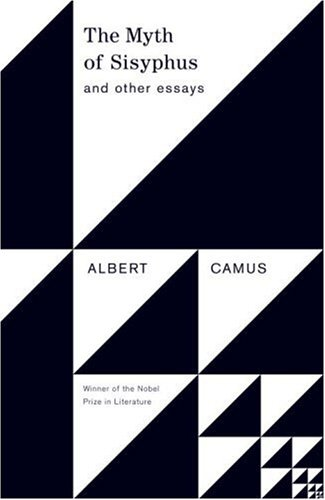
\includegraphics[width=0.22\textwidth]{the-myth-of-sisyphus-cover.jpg}}
\label{fig:3844X0}
\end{floatingfigure} In 1942, with World II raging, readers of
\href{http://www.amazon.com/Myth-Sisyphus-Other-Essays/dp/0679733736}{The
Myth of Sisyphus} could easily identify with Camus's absurd man. Not
only is man absurd he has reduced his entire world to absurdity. Now,
seventy-plus years later, Sisyphus readers are more likely to politely
yawn and wonder what the fuss is about. Camus's themes are not trivial
or obvious but we, denizens of the early 21\textsuperscript{st} century,
are thoroughly habituated to them. Absurd is now beyond mainstream; how
else can one explain facile growths like Facebook. Just like homosexuals
kidnapped the word ``gay'' and changed its meaning Camus abducted
``absurd'' and changed its meaning. The old ``absurd'', synonymous with
ridiculous, nonsensical, ludicrous and preposterous, becomes, in Camus's
hands, something few would call absurd. But, part of a great writer's
job description is changing the meaning of words, and it's easy to see
why the best of us have become absurd men.

Camus's absurd man is a thoroughly honorable creature. He respects
reason and wants to understand all things. This is beyond his reach but
he doesn't claim it's impossible, only that his own limits make it
\emph{personally} impossible. Perhaps you've vainly argued with
scientific illiterates that assert evolution is wrong because
\emph{they} cannot see how it could work. \emph{If I don't understand it
then it cannot be understood}. Absurd men recognize, but do not
generalize, their limitations. Absurd men also see that in the long run
absolutely nothing matters. In a thousand years all but the greatest of
us will be forgotten, in a million years even the greatest will be
forgotten, in a billion years only precision instruments will detect our
remains and in a trillion years it will be like we never existed. Many
red dwarf stars will still be shining long after every microscopic trace
of humanity has disappeared. This is an inescapable scientific truth.
It's a terrifying banality that is often ignored or wrapped up in sky
fairy nonsense. Yet, the absurd man faces cosmic futility without
flinching or whining.

Instead of being crushed by a vast, difficult to comprehend, cosmos the
absurd man soldiers on. He doesn't curl up, go on food stamps, or
complain about lurid Koch brother conspiracies. He gives a middle finger
to his fate and then does what he can. \emph{Up yours universe:} this is
Camus's \emph{revolt} and, in our time, it's a universal sentiment. This
part of being absurd is easily faked; every brain-dead rapper and
air-headed celebrity sports \emph{up-yours-airs,} but absurd men do not
play at revolt! They do their best to create without delusions and what
idiot would claim celebrities are free of delusions? Many like to think
cathedral masons were honoring god. Even in the Middle Ages this was
delusional. Most were simply earning a living: if a pile of well-shaped
rocks pleased god who knew or cared. Besides, in a geological blink, the
same cathedral stones will weather~to mud. Camus is very clear: absurd
creation is self-consciously ephemeral.

Camus started The Myth of Sisyphus with what's become his most famous
line:

\begin{quotation}
    \emph{There is but one truly serious philosophical problem and that is suicide.}
\end{quotation}

This is one exam question we all face. Cowards run and hide; they turn
the knob to eleven and pop sweet --- there's an app for that ---
distractions. The religious create elaborate fantasies and declare war.
Pure rationalists drag in Spinoza's objects that long to persist in
their being. They don't commit suicide because that's not part of their
program. Ironically, only Camus's absurd answer is remotely satisfying.
In our lingo: man-up, stop whining, pull your weight, don't take crap,
expect nothing, use your head and create. Any modern libertarian would
approve.


\begin{floatingfigure}[r]{0.24\textwidth}
\centering
\href{http://www.wikipaintings.org/en/titian/sisyphus-1549}{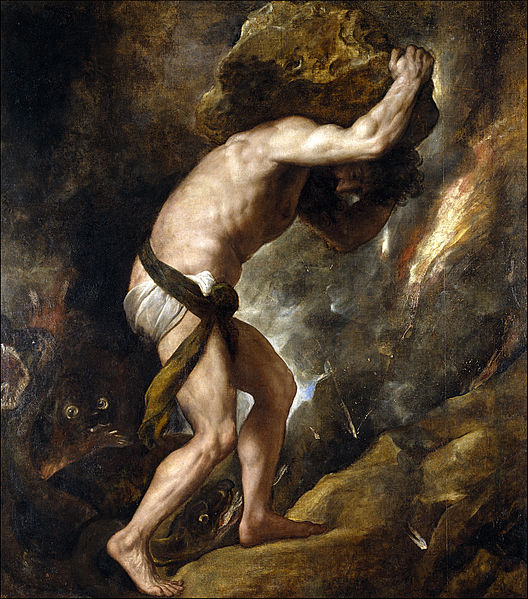
\includegraphics[width=0.23\textwidth]{sisyphus-rocking-it.jpg}}
\label{fig:3844X1}
\end{floatingfigure} When
casting the prototypical absurd man Camus brilliantly chose Sisyphus.
Sisyphus put death in chains, claiming immortality for men, but vindictive
and jealous gods freed death and condemned Sisyphus to roll a heavy
stone to the top of a hill only to watch it crash down and roll it
up again, and~again~--- forever. This sounds awful but Camus saw
Sisyphus's fate as a blessing. Life sucks when you're pushing your rock
up the hill but when it rolls down you get a break. While climbing down
Sisyphus has time to think, to absurdly create, and unlike poor
doomed mortals, Sisyphus gets an eternity of breaks. This is an absurdly
happy fate.

%\captionsetup[floatingfigure]{labelformat=empty}
%\begin{figure}[htbp]
%\begin{floatingfigure}[l]{0.25\textwidth}
%\centering
%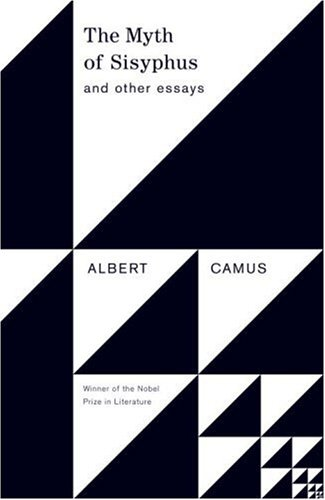
\includegraphics[width=0.23\textwidth]{the-myth-of-sisyphus-cover.jpg}
%\caption{~~~IMCAPTION~~~}
%\label{fig:3844X0}
%\end{floatingfigure}
%\end{figure}

%\captionsetup[floatingfigure]{labelformat=empty}
%\begin{figure}[htbp]
%\begin{floatingfigure}[l]{0.25\textwidth}
%\centering
%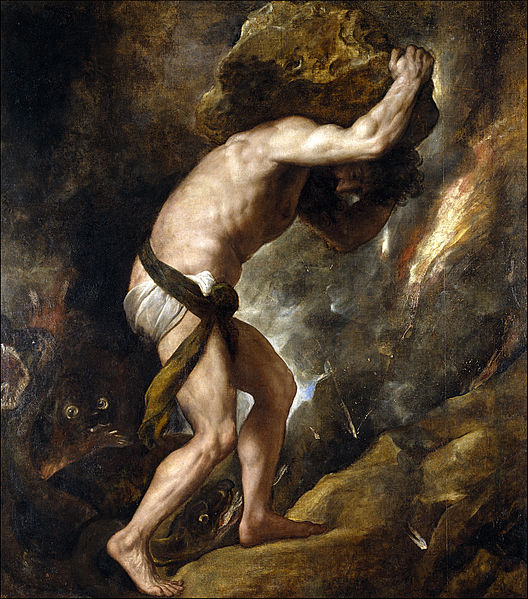
\includegraphics[width=0.23\textwidth]{sisyphus-rocking-it.jpg}
%\caption{~~~IMCAPTION~~~}
%\label{fig:3844X1}
%\end{floatingfigure}
%\end{figure}



%\end{document}